%!TEX root=./paper.tex
\subsection{Results}

\begin{figure*}[]
  \centering
  \begin{subfigure}[b]{0.9\textwidth}
      \centering
      \includegraphics[width=\textwidth]{mape_pred.eps}
      \caption{MAPE on prediction task for different deltas}
      \label{fig:mape_pred}
  \end{subfigure}
  
  \begin{subfigure}[b]{0.9\textwidth}
      \centering
      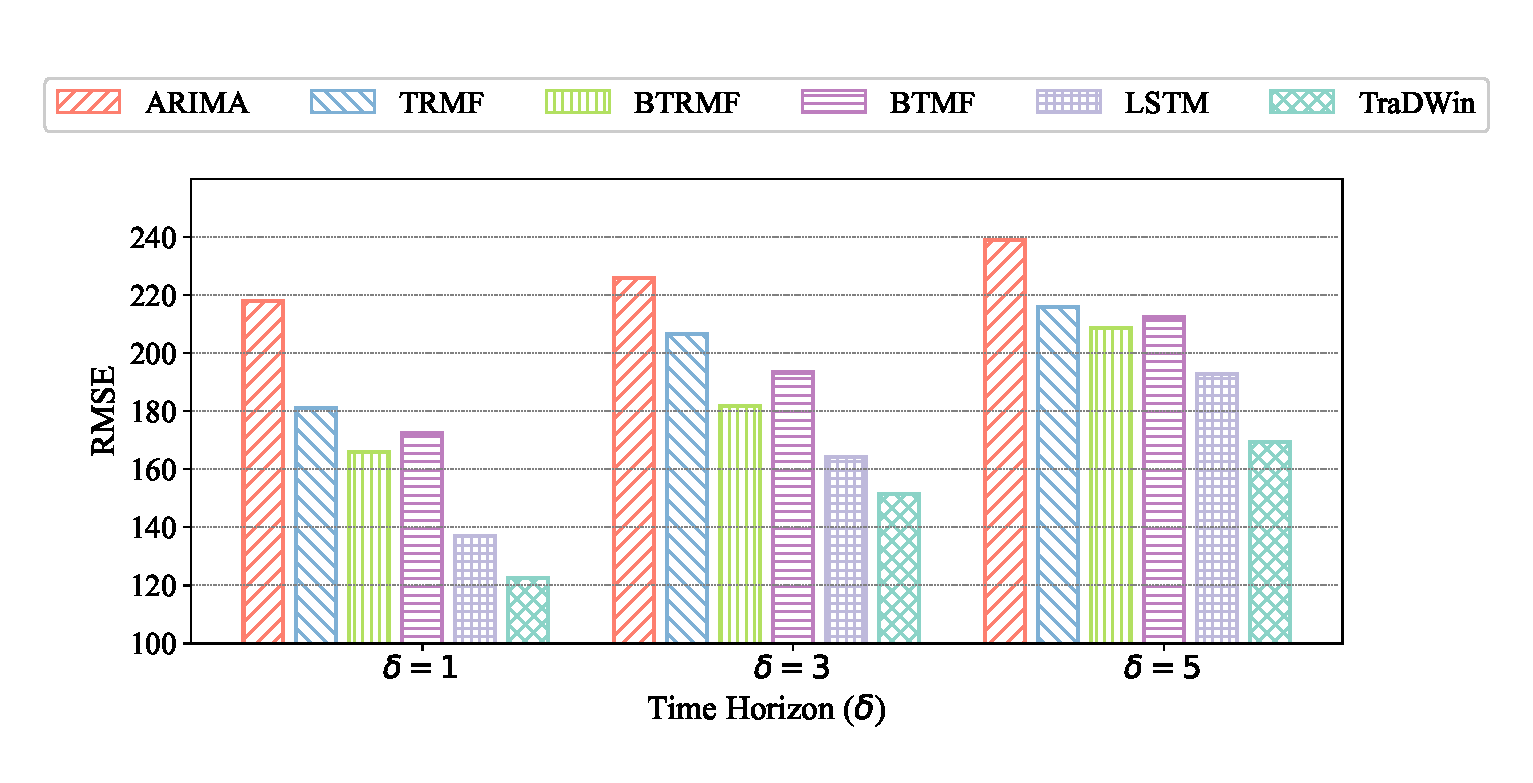
\includegraphics[width=\textwidth]{rmse_pred.eps}
      \caption{RMSE on prediction task for different deltas}
      \label{fig:rmse_pred}
  \end{subfigure}
  
  \caption{Performance metrics on prediction task for different deltas (timesteps to predict ahead)}
  \label{fig:pred_metrics}
\end{figure*}

We evaluated the performance of our model on different tasks and compared them with other popular models used in the domain. For the prediction task, we tested the models for predicting traffic volumes at the next timestep, i.e., the forecasting $\delta = 1$, at the third timestep, i.e., $\delta = 3$ and the fifth timestep in the future, i.e., $\delta = 5$. This scenario of predicting the next time step requires a mask consisting of all the $T_{n+1}$ values missing, i.e., 0. We prepare a mask similarly for other time horizons. Thus, the prediction here is treated as a strict MNAR (Missing Not At Random) subcategory of imputation.

The MAPE and RMSE plots of prediction tasks on different horizons are shown in Fig. \ref{fig:mape_pred} and Fig. \ref{fig:rmse_pred}, respectively. We observe that in general, as the $\delta$, i.e., the time horizon to predict in the future, increases, both metrics worsen with MAPE falling 5-10\% from $\delta=1$ to $\delta=3$, i.e., we see a stronger short term accuracy but face some challenges with long-term prediction, across all models. This trend is common in time-series forecasting, where predictive accuracy decreases as the prediction horizon extends. The primary reasons for this decline include the increasing uncertainty and the influence of unpredictable external factors, such as accidents or weather changes. We see that ARIMA performs worst, which is to be expected since it is the simplest of mathematical models among the baselines we consider. The other matrix factorization and Bayesian models like TRMF, BTRMF, and BTMF perform better, but given that they are strictly mathematical models, they (i) fail to capture the intricate traffic dynamics that a deep learning model can and (ii) use only the time-series traffic data and not the graph topology and external factors that our model considers like weather, etc. Finally, we see that LSTMs are close with slightly (2-3\%) worse performance, which could be attributed to a lack of knowledge of graph topology that we incorporate in our model through $Node2Vec$. Overall, we see that our \name\ model performs significantly better than most models, scoring roughly 3 to 7 percentage points better than the baselines.

\begin{figure*}[]
\centering
\begin{subfigure}{0.5\textwidth}
  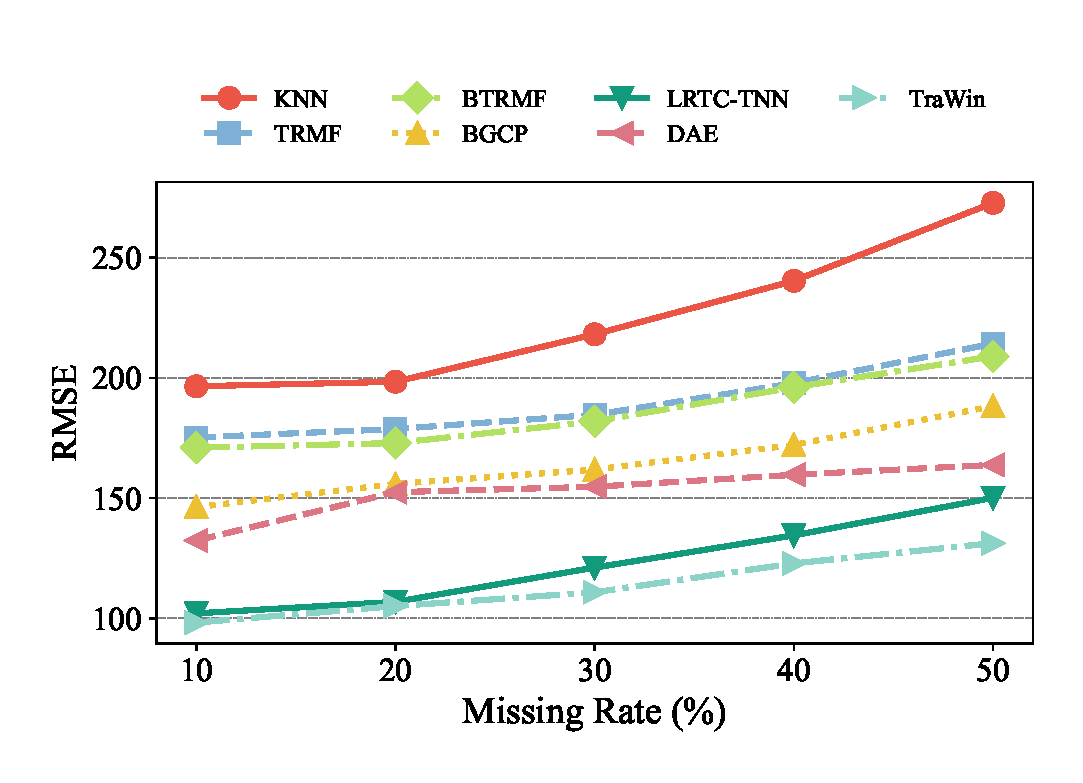
\includegraphics[width=\linewidth]{rmse_imput.eps}
  \caption{RMSE of different models on imputation task}
  \label{fig:mape_imput}
\end{subfigure}%
\begin{subfigure}{0.5\textwidth}
  \includegraphics[width=\linewidth]{mape_imput.eps}
  \caption{MAPE of different models on imputation task}
  \label{fig:rmse_imput}
\end{subfigure}
\caption{Imputation comparison for different missing rates}
\label{fig:imput}
\end{figure*}

Next, we evaluate performance on the imputation task. For this task, we have considered the MCAR (Missing Completely At Random) distribution and compared the models at five missing rates of $10\%$, $20\%$, $30\%$, $40\%$, and $50\%$. The performance of different models measured using MAPE and RMSE is shown in Fig. \ref{fig:imput}. We see that the conventional methods, like KNN, perform poorly to more specialized approaches, which is to be expected since KNN is not enough to capture the intricate traffic dynamics. The matrix factorization and Bayesian methods, which are TRMF, BTRMF, and BGCP, work slightly better, with deep learning methods like DAE following ahead, though since they deal with only traffic data time series with no information on topology, they have an 8-13\% worse off performance than our model. Tensor completion based model like LRTC-TNN is close to our \name\ for low missing rates, but we see that it does not scale as well with increasing missing rates, possibly because too much data is lost for reliable tensor completion, which a deep learning model can still handle, due to being able to learn more complex relationships in data and having knowledge of graph topology and other external factors. Moreover, it is worth noting that LRTC-TNN is an MCAR imputer and not applicable to task (iii), so it is not generalized enough for our use case. For all models, we see that the accuracy of imputations decreases with higher missing rates due to the reduced amount of contextual information available. This is a common challenge in data imputation, where fewer data points make it harder to discern underlying patterns accurately. Overall, we observe that \name\ scales well with more missing data and is significantly (5-7\%) better than the compared baselines.


\begin{figure}[t]
  \centering
  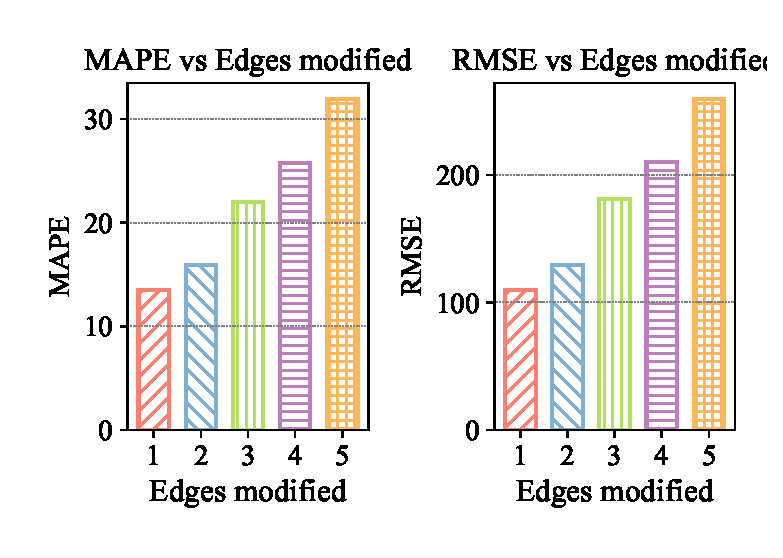
\includegraphics[width=\linewidth]{modif.eps}
  \caption{MAPE and RMSE on re-assignment task vs number of edges modified}
  \label{fig:edge_modif}
\end{figure}

We also observe that \name\ performs better on task (ii) than on task (i) by around 4\%. One primary reason for this, as we suspect, could be that GAIN, which was originally designed for MCAR (Missing Completely At Random) imputation, does not generalize well to MNAR imputation scenarios. Another possible reason could be the subgraph-based computation method that we use, where nodes at the corners of the subgraph do not have adequate spatial and temporal information about their neighbors. Overall, we observe that our model performs reasonably and delivers comparable results for being a generalized model on both tasks.

Finally, on the re-assignment task, which is a new task that we address in our paper and is not conventionally seen in contemporary literature, we essentially train the model for MNAR (Missing Not At Random) imputation scenarios with the central node cluster missing. This effectively makes the model learn how to assign traffic to node clusters given neighbor node information. To elaborate further, for an edge that is modified, nodes around the edge, based on a distance threshold, are masked, i.e., marked missing. For training input, the features for the neighbors of the cluster (nodes not masked out, but around the cluster), graph embeddings for the masked nodes (not the traffic volume as that is marked missing), and the total volume of traffic for the masked out nodes is given. The task is then to assign traffic volumes to the masked-out nodes and compare them against what they were originally. The idea was for the model to learn "traffic assignment", since we can't have real world labeled data for traffic state before and after modification of edges. Based on this training task, we achieved a MAPE of $13.47\%$ and RMSE of $109.90$. Note that the other baselines considered for prediction and imputation are not applicable to this without changes to their model architecture, so there is no comparison with contemporary models.

Further, the de-facto way to solve this problem, as we have seen in our literature review, has been simulations like SUMO\cite{sumo} and Vissim\cite{vissim}. Using SUMO, a traffic simulation, we also use those to compare and test our model on the TAPASCologne scenario. We train using the same approach as for the Dublin SCATS dataset but test against the simulation results after modification of the said edge.  This is not possible for the Dublin dataset since we don't have detailed origin-destination pair data for it. The results of our model on this task are shown in Table \ref{reassign_table}. We observe that the model achieves a MAPE of $13.47\%$ on the Dublin SCATS dataset and $15.06\%$ on the TAPASCologne scenario, which demonstrates that the model can, with reasonable accuracy, learn to solve the traffic assignment problem on node clusters. Further, we tried to evaluate how our model's performance scales with the number of modifications, i.e., how much we can alter the original graph so that the model is still viable to use for re-assignment. In Fig. \ref{fig:edge_modif}, we show a comparison of MAPE and RMSE with the number of edges modified. We see that performance declines steadily from $13.47\%$ at $1$ change to $31.91\%$ at 5 changes. So, altering more of the graph leads to a decline in performance, with the drop being significant and sharp after $3$ modifications. A possible reason for this could be the mass masking strategy we use to train the model for task (iii). For 5 modifications, too many of the neighboring nodes are masked, leading to a large loss of contextual information that knowledge of graph representation does not compensate enough. 

\begin{table}[]
\centering
\caption{Performance on re-assignment task (1 edge change) for different datasets}
\label{reassign_table}
\begin{tabular}{lcc}
\toprule
Dataset & MAPE (\%) & RMSE \\
\midrule
Dublin SCATS & 13.47 & 109.90 \\
TAPASCologne & 15.06 & 23.34 \\
\bottomrule
\end{tabular}
\end{table}